%!TEX root = ../EDC_Part_II_Weak_Sector_rebuild.tex
% ==============================================================================
% OPR-20b Attempt H2 — HARD MODE AUDIT: δ = R_ξ Provenance
% Status: RIGOROUS AUDIT — two-route derivation attempt or honest downgrade
% Version: 1.0 (2026-01-23)
% ==============================================================================
%
% MISSION (H2-HARD):
% Either (i) produce a real two-route derivation to upgrade δ = R_ξ to [Dc],
% or (ii) formally downgrade and restructure with explicit gates and failure modes.
%
% ABSOLUTE CONSTRAINTS:
% - NO modification of existing equations, labels, refs, numeric values
% - Every new paragraph must end with an epistemic tag: [P], [Dc], [I], [BL], [M], [OPEN]
% - No SM-smuggling: M_W, M_Z, v, sin²θ_W, G_F may not be used as sources
%
% ==============================================================================

\subsection{Attempt H2 (Hard Mode): Rigorous Audit of \texorpdfstring{$\delta = R_\xi$}{delta = Rxi} Provenance}
\label{sec:ch11_opr20_attemptH2_hard}

% ------------------------------------------------------------------------------
% (1) TITLE + WHAT WE ARE TRYING TO PROVE
% ------------------------------------------------------------------------------

\subsubsection{Objective: What We Are Trying to Prove}
\label{sec:H2hard_objective}

The Robin boundary condition that emerges from thick-brane variation has the form
$f' + \alpha f = 0$, where on dimensional grounds $\alpha \sim \ell/\delta$.
Here $\ell$ is the orbifold circumference and $\delta$ is an effective
``boundary-layer thickness''---the scale over which fields transition from
bulk-dominated to brane-dominated behavior. \tagM{}

The identification $\delta = R_\xi$ (where $R_\xi$ is the membrane correlation
length from Part~I) would close a critical gate in the G$_F$ derivation chain.
This audit applies \textbf{two independent derivation routes} to determine whether
this identification can be upgraded from postulate [P] to derived-conditional [Dc].
If neither route succeeds, the identification must remain [P] with explicit
upgrade conditions documented. \tagM{}

\begin{tcolorbox}[colback=blue!5!white, colframe=blue!60!black,
    title=\textbf{Precise Statement (H2-Hard Target)}]
\textbf{Goal:} Prove or disprove that the boundary-layer thickness $\delta$
(entering $\alpha = \ell/\delta$) equals the membrane correlation length $R_\xi$
(from Part~I diffusion dynamics), using only EDC microphysics. \tagM{}

\textbf{Success criterion:} Two independent derivation routes converge to
$\delta = c \cdot R_\xi$ with a derived dimensionless constant $c$. \tagM{}

\textbf{Failure criterion:} If either route is blocked or the final step
requires postulation, the identification remains [P]+[OPEN]. \tagM{}
\end{tcolorbox}

% ------------------------------------------------------------------------------
% (2) KNOWN DEFINITIONS (ALLOWED) BOX
% ------------------------------------------------------------------------------

\subsubsection{Known Definitions (Allowed)}
\label{sec:H2hard_definitions}

\begin{tcolorbox}[colback=gray!5!white, colframe=gray!60!black,
    title=\textbf{Definition Block: Allowed Inputs}]

\textbf{Definition D1: Boundary-layer thickness $\delta$} \tagDef{}

The boundary-layer thickness $\delta$ is the characteristic length scale over
which a field transitions from its bulk behavior to its brane-localized behavior.
In the Robin BC context, $\alpha \equiv \ell/\delta$ (up to $\mathcal{O}(1)$
geometric factors). \tagDef{}

\textbf{Where used:} Thick-brane BVP (§11--12), Robin BC derivation,
mediator mass calculation.

\medskip
\textbf{Definition D2: Membrane correlation length $R_\xi$} \tagDef{}+\tagBL{}

From Part~I (Framework v2.0): $R_\xi$ is the correlation length of the frozen
membrane, defined via $\langle \phi(x)\phi(x') \rangle \sim e^{-|x-x'|/R_\xi}$.
It characterizes the spatial scale of diffusion/relaxation in the frozen regime.
\tagDef{}

\textbf{Numerical value:} $R_\xi \approx 2 \times 10^{-3}$ fm, constrained by
electroweak observables ($R_\xi = \hbar c / M_Z$). \tagBL{}+\tagP{}

\textbf{Critical note:} The \emph{value} of $R_\xi$ is phenomenologically
constrained [P]+[BL], not derived from the EDC action. Deriving $R_\xi$ from
first principles is an open problem (see OPR-20c below). \tagP{}

\medskip
\textbf{Definition D3: Orbifold circumference $\ell$} \tagDc{}

From KK geometry: $\ell = 2\pi R_\xi$ is the circumference of the compact
dimension. The factor $2\pi$ comes from standard circle geometry (radius
$\to$ circumference). This is derived. \tagDc{}

\end{tcolorbox}

% ------------------------------------------------------------------------------
% (3) FORBIDDEN MOVES (SMUGGLING GUARDRAIL) BOX
% ------------------------------------------------------------------------------

\subsubsection{Forbidden Moves (Smuggling Guardrail)}
\label{sec:H2hard_forbidden}

\begin{tcolorbox}[colback=red!5!white, colframe=red!60!black,
    title=\textbf{No-Smuggling Guardrail: Forbidden Moves}]

The following are \textbf{explicitly forbidden} in any derivation of
$\delta = R_\xi$. Violation of these rules invalidates any [Dc] claim. \tagDc{}

\begin{enumerate}[nosep]
    \item \textbf{SM observable fitting:} Using $M_Z$, $M_W$, $v$, $\sin^2\theta_W$,
          $g$, $g'$, or $G_F$ to \emph{determine} $\delta$ or $R_\xi$. These may
          only appear in a \emph{consistency check} box (not a derivation). \tagDc{}

    \item \textbf{Reverse-engineering:} Picking $\delta$ to achieve a
          desired $\alpha$ range (e.g., $\alpha \in [5.5, 15]$) without
          independent derivation. \tagDc{}

    \item \textbf{Profile ansatz assumption:} Assuming $f(\xi) \propto e^{-\xi/\delta}$
          \emph{a priori} and then extracting $\delta$ from this ansatz. \tagDc{}

    \item \textbf{``Only available scale'' without proof:} Claiming $R_\xi$
          is the unique transverse scale without formally excluding alternatives
          (e.g., $\bar\lambda_e$, $r_e$, ratio combinations). \tagDc{}

    \item \textbf{Circular parameter definition:} Defining $\delta \equiv R_\xi$
          as a postulate and then claiming the equality is ``derived.'' \tagDc{}

    \item \textbf{$\mathcal{O}(1)$ adjustment:} Introducing dimensionless factors
          (e.g., $c = 0.9$, $c = 1.2$) selected to reproduce SM observables. \tagDc{}
\end{enumerate}
\end{tcolorbox}

% ------------------------------------------------------------------------------
% (4) ROUTE A: DIFFUSION/TRANSPORT → BOUNDARY LAYER THICKNESS δ
% ------------------------------------------------------------------------------

\subsubsection{Route A: Diffusion/Transport $\to$ Boundary-Layer Thickness $\delta$}
\label{sec:H2hard_routeA}

\paragraph{Required derivation chain.}
Route A would derive $\delta$ from the diffusion dynamics of the membrane
using matched asymptotic expansions or boundary-layer theory from PDEs. \tagM{}

\textbf{Step A1:} Identify the diffusion PDE in Part~I that governs
membrane fluctuations. Candidate: $\partial_t \phi = D \nabla^2 \phi - V'(\phi)$
in the frozen regime. \tagM{}

\textbf{Step A2:} Apply boundary-layer analysis near the brane ($\xi \to 0$).
The inner solution (near brane) must match the outer solution (bulk) at
an overlap region of thickness $\delta_{\text{BL}}$. \tagM{}

\textbf{Step A3:} Extract $\delta_{\text{BL}}$ as a function of diffusion
parameters: $\delta_{\text{BL}} = f(D, \tau, V''(\phi_0), ...)$. \tagM{}

\textbf{Step A4:} Show that $\delta_{\text{BL}} = R_\xi$ using Part~I
definitions of $D$ and $\tau$. \tagM{}

\paragraph{Audit of Step A1.}

\begin{tcolorbox}[colback=yellow!5!white, colframe=yellow!60!black,
    title=\textbf{Route A1 Status}]
\textbf{Diffusion PDE in Part I:} EXISTS (frozen membrane regime). \tagDc{}

The Part~I action yields a diffusion-like equation for membrane fluctuations
in the frozen regime. The diffusion coefficient $D$ and correlation time
$\tau$ are defined. However, these are 4D quantities---the transverse ($\xi$)
direction is not explicitly treated. \tagDc{}

\textbf{Finding:} Diffusion PDE exists, but is 4D (membrane), not 5D (bulk).
The transverse direction is implicit. \tagDc{}
\end{tcolorbox}

\paragraph{Audit of Step A2.}

\begin{tcolorbox}[colback=red!5!white, colframe=red!50!black,
    title=\textbf{Route A2 Status: BLOCKED}]
\textbf{Boundary-layer analysis:} DOES NOT EXIST in current repo. \tagOPEN{}

A proper matched-asymptotic analysis would require:
\begin{itemize}[nosep]
    \item Inner expansion near $\xi = 0$ (brane region)
    \item Outer expansion for $\xi \gg \delta$ (bulk region)
    \item Matching condition at $\xi \sim \delta$
\end{itemize}

This analysis has not been performed. It represents genuine future work,
not a gap that can be filled by reformulation. \tagOPEN{}
\end{tcolorbox}

\paragraph{Audit of Steps A3--A4.}

\begin{tcolorbox}[colback=red!5!white, colframe=red!50!black,
    title=\textbf{Route A3--A4 Status: BLOCKED}]
\textbf{$\delta_{\text{BL}}$ extraction:} CANNOT PROCEED without A2. \tagOPEN{}

\textbf{$\delta_{\text{BL}} = R_\xi$ proof:} CANNOT PROCEED without A3. \tagOPEN{}

Without the boundary-layer theorem, there is no rigorous derivation of
$\delta$ from diffusion dynamics. The chain is broken at Step A2. \tagOPEN{}
\end{tcolorbox}

\paragraph{Route A Verdict.}

\begin{tcolorbox}[breakable, enhanced, colback=red!5!white, colframe=red!70!black,
    title=\textbf{Route A Verdict: BLOCKED}, width=\linewidth]
\textbf{Status:} Route A is \textbf{BLOCKED} at Step A2. \tagOPEN{}

\textbf{What exists:}
\begin{itemize}[nosep]
    \item Diffusion PDE in Part~I (frozen regime) \tagDc{}
    \item Correlation length $R_\xi$ definition \tagDef{}
\end{itemize}

\textbf{What is missing:}
\begin{itemize}[nosep]
    \item Transverse ($\xi$-direction) diffusion equation \tagOPEN{}
    \item Matched asymptotic analysis \tagOPEN{}
    \item Boundary-layer theorem \tagOPEN{}
    \item Proof that $\delta_{\text{BL}} = R_\xi$ \tagOPEN{}
\end{itemize}

\textbf{Conclusion:} Route A cannot produce $\delta = R_\xi$ in the
current state of the theory. This is a genuine gap (OPR-20d). \tagOPEN{}
\end{tcolorbox}

% ------------------------------------------------------------------------------
% (5) ROUTE B: JUNCTION/VARIATION → ROBIN BC → δ
% ------------------------------------------------------------------------------

\subsubsection{Route B: Junction/Variation $\to$ Robin BC $\to$ $\delta$}
\label{sec:H2hard_routeB}

\paragraph{Required derivation chain.}
Route B would derive $\delta$ from the junction conditions that produce
the Robin boundary condition. \tagM{}

\textbf{Step B1:} Start from 5D action with brane boundary (Israel matching
or Gibbons-Hawking-York boundary term). \tagM{}

\textbf{Step B2:} Vary the action to obtain the junction condition on fields:
the Israel matching relates field discontinuities to brane stress-energy. \tagM{}

\textbf{Step B3:} Map the junction condition to Robin BC form:
$f' + \alpha f = 0$ with $\alpha$ expressed in terms of junction parameters. \tagM{}

\textbf{Step B4:} Identify the dimensional structure $\alpha \sim \ell/\delta$
to extract $\delta$ from $\alpha$. \tagM{}

\textbf{Step B5:} Show that this $\delta$ equals $R_\xi$ using Part~I
definitions---without SM input. \tagM{}

\paragraph{Audit of Steps B1--B3.}

\begin{tcolorbox}[colback=green!5!white, colframe=green!60!black,
    title=\textbf{Route B1--B3 Status: DERIVED}]
\textbf{5D action with brane boundary:} EXISTS (thick-brane variation). \tagDc{}

\textbf{Junction $\to$ Robin mapping:} DERIVED in Attempts F/G. \tagDc{}

From the boundary action variation:
\begin{equation}
    S_{\text{brane}} = \int d^4x \left[ -\frac{\kappa}{2}\phi^2 +
    \text{(kinetic terms)} \right]
\end{equation}
the field equation yields Robin BC: $f'(z_0) + \alpha\cdot f(z_0) = 0$.
The Robin \emph{structure} emerges from action variation, not postulation. \tagDc{}
\end{tcolorbox}

\paragraph{Audit of Step B4.}

\begin{tcolorbox}[colback=green!5!white, colframe=green!60!black,
    title=\textbf{Route B4 Status: DERIVED}]
\textbf{Dimensional structure $\alpha \sim \ell/\delta$:} DERIVED. \tagDc{}

On dimensional grounds, $\alpha$ has dimension [1/length]. The natural
structure is $\alpha = c_{\text{geom}} \cdot \ell / \delta$ where $c_{\text{geom}}$
is an $\mathcal{O}(1)$ geometric factor. This is a mathematical consequence
of the dimensional analysis, not a postulate. \tagDc{}

From this, $\delta = c_{\text{geom}} \cdot \ell / \alpha$. To extract $\delta$,
we need either (i) the value of $\alpha$ from physics, or (ii) the
identification of $\delta$ with a known scale. \tagDc{}
\end{tcolorbox}

\paragraph{Audit of Step B5.}

\begin{tcolorbox}[colback=red!5!white, colframe=red!50!black,
    title=\textbf{Route B5 Status: INCOMPLETE}]
\textbf{$\delta = R_\xi$ derivation:} NOT ACHIEVED. \tagP{}

The junction variation gives the Robin BC structure and $\alpha \sim \ell/\delta$,
but does \emph{not} uniquely determine $\delta$. Two possibilities exist:

\begin{enumerate}[nosep]
    \item \textbf{Physical identification:} Assert $\delta = R_\xi$ because
          ``both characterize relaxation scales.'' This is a plausibility
          argument, not a derivation. \tagP{}

    \item \textbf{Action-derived $\alpha$:} Compute $\alpha$ from the brane
          tension/BKT coefficient and invert to get $\delta$. This requires
          knowing $\kappa$ or $\lambda$ from EDC physics. \tagOPEN{}
\end{enumerate}

\textbf{Current state:} We use Option 1 (physical identification) in the book.
This is a postulate [P], not a derivation [Dc]. \tagP{}
\end{tcolorbox}

\paragraph{Route B Verdict.}

\begin{tcolorbox}[breakable, enhanced, colback=yellow!5!white, colframe=yellow!60!black,
    title=\textbf{Route B Verdict: PARTIAL}, width=\linewidth]
\textbf{Status:} Route B is \textbf{PARTIAL}. \tagDc{}+\tagP{}

\textbf{What is derived [Dc]:}
\begin{itemize}[nosep]
    \item Robin BC structure from action variation \tagDc{}
    \item $\alpha \sim \ell/\delta$ dimensional structure \tagDc{}
    \item $\ell = 2\pi R_\xi$ circumference relation \tagDc{}
\end{itemize}

\textbf{What is postulated [P]:}
\begin{itemize}[nosep]
    \item $\delta = R_\xi$ identification (physical plausibility) \tagP{}
    \item Therefore: $\alpha = \ell/\delta = 2\pi$ (inherits [P]) \tagP{}
\end{itemize}

\textbf{What is open [OPEN]:}
\begin{itemize}[nosep]
    \item Derive $\alpha$ from action parameters (BKT, tension) \tagOPEN{}
    \item Unique transverse scale theorem \tagOPEN{}
\end{itemize}

\textbf{Conclusion:} Route B establishes the structure but the final
$\delta = R_\xi$ step is assumed, not derived. Cannot upgrade to [Dc]. \tagP{}
\end{tcolorbox}

% ------------------------------------------------------------------------------
% (6) CONVERGENCE TEST
% ------------------------------------------------------------------------------

\subsubsection{Convergence Test: Do Routes A and B Agree?}
\label{sec:H2hard_convergence}

\begin{tcolorbox}[colback=red!5!white, colframe=red!70!black,
    title=\textbf{Convergence Test: CANNOT BE PERFORMED}]

\textbf{Route A status:} BLOCKED (boundary-layer theorem missing) \tagOPEN{}

\textbf{Route B status:} PARTIAL (final $\delta = R_\xi$ step is [P]) \tagP{}

\textbf{Convergence test result:} \textcolor{BrickRed}{\textbf{CANNOT BE PERFORMED}} \tagOPEN{}

Without two independent derivations, there is nothing to compare.
The ``$\delta = R_\xi$'' identification rests on a single plausibility
chain (Route B), not on convergent derivations. \tagOPEN{}

\medskip
\textbf{What would constitute convergence:}
\begin{itemize}[nosep]
    \item Route A: $\delta_{\text{BL}} = \sqrt{D\tau}$ from matched asymptotics
    \item Route B: $\delta = \ell/\alpha$ with $\alpha$ derived from action
    \item Convergence: $\sqrt{D\tau} = \ell/\alpha = R_\xi$ (all routes agree)
\end{itemize}

\textbf{Current gap:} Route A blocked; Route B incomplete. No convergence possible. \tagOPEN{}
\end{tcolorbox}

% ------------------------------------------------------------------------------
% (7) SINGLE SENTENCE RULE BOX
% ------------------------------------------------------------------------------

\subsubsection{Single Sentence Rule: Canonical Statement}
\label{sec:H2hard_single_sentence}

\begin{tcolorbox}[colback=blue!5!white, colframe=blue!70!black,
    title=\textbf{Single Sentence Rule (Book-Ready)}]

Based on the H2-Hard audit, the book is authorized to make \textbf{exactly one}
of the following canonical statements. \tagDc{}

\medskip
\textbf{Option 1 (if NOT derived):}
\begin{quote}
\textit{``We postulate $\delta \equiv R_\xi$ as the membrane thickness scale;
deriving this identity from brane microphysics remains an explicit open problem
(OPR-20b, OPR-20d).''} \tagP{}+\tagOPEN{}
\end{quote}

\textbf{Option 2 (if derived via Route A+B convergence):}
\begin{quote}
\textit{``From matched asymptotic analysis of the membrane diffusion equation
[Route A] and junction variation [Route B], the boundary-layer thickness
$\delta = R_\xi$ follows, identifying the Robin parameter $\alpha = 2\pi$.''} \tagDc{}
\end{quote}

\medskip
\fcolorbox{red}{yellow!20}{\parbox{0.9\textwidth}{
\textbf{H2-Hard Verdict:} The derivation is \textbf{NOT complete}. \\
The book must use \textbf{Option 1} (postulated). \\
Option 2 is \textbf{NOT authorized} until OPR-20d is closed.
}}
\end{tcolorbox}

% ------------------------------------------------------------------------------
% (8) FAILURE MODES BOX
% ------------------------------------------------------------------------------

\subsubsection{Failure Modes}
\label{sec:H2hard_failure_modes}

\begin{tcolorbox}[breakable, enhanced, colback=orange!5!white, colframe=orange!60!black,
    title=\textbf{Failure Modes: How $\delta = R_\xi$ Could Be Wrong}, width=\linewidth]

The following failure modes must be monitored. If any is triggered, the
identification $\delta = R_\xi$ is falsified or must be modified. \tagDc{}

\begin{enumerate}
    \item[\textbf{FM-H2-1}:] \textbf{$\delta$ is not unique.} Multiple microscopic
          lengths exist ($\bar\lambda_e$, $r_e$, $r_e^2/R_\xi$, etc.), and
          there is no principle selecting $R_\xi$. Without a uniqueness
          theorem, the identification is ambiguous. \tagOPEN{}

    \item[\textbf{FM-H2-2}:] \textbf{$\delta$ depends on energy/field species.}
          Different fields (fermion vs. scalar vs. gauge) may have different
          boundary-layer thicknesses. A universal $\delta$ may not exist. \tagOPEN{}

    \item[\textbf{FM-H2-3}:] \textbf{$\delta$ and $R_\xi$ are different objects.}
          $\delta$ is a boundary-layer width (transverse). $R_\xi$ is a
          correlation length (4D membrane). They may not be the same
          geometric object. \tagOPEN{}

    \item[\textbf{FM-H2-4}:] \textbf{$\alpha$ derived but $\delta$ not extractable.}
          The junction physics may give $\alpha$ in terms of brane tension
          $\sigma$ or BKT $\lambda$, but the relation $\alpha = \ell/\delta$
          may not hold (different geometric structure). \tagOPEN{}

    \item[\textbf{FM-H2-5}:] \textbf{Diffusion model absent.} The frozen-regime
          diffusion equation does not extend to the transverse direction,
          so ``diffusion scale = boundary layer'' is an analogy, not a
          derivation. \tagOPEN{}

    \item[\textbf{FM-H2-6}:] \textbf{Circularity via EW scale.} If $R_\xi$
          is defined as $\hbar c / M_Z$, then any ``derivation'' of
          $\delta = R_\xi$ that relies on EW observables is circular.
          The identification would be [I] (fit), not [Dc] (derived). \tagOPEN{}
\end{enumerate}

\textbf{Current status:} FM-H2-5 and FM-H2-6 are \emph{partially triggered}.
Route A is blocked (FM-H2-5), and $R_\xi$ value comes from EW phenomenology
(FM-H2-6 as warning). \tagOPEN{}
\end{tcolorbox}

% ------------------------------------------------------------------------------
% (9) UPGRADE GATES BOX
% ------------------------------------------------------------------------------

\subsubsection{Upgrade Gates: Path to [Dc]}
\label{sec:H2hard_upgrade_gates}

\begin{tcolorbox}[colback=green!5!white, colframe=green!60!black,
    title=\textbf{Upgrade Gates (OPR-20c/d/e)}]

The following gates must be closed to upgrade $\delta = R_\xi$ from [P] to [Dc].
Each gate specifies: required input, expected artifact, and what it unlocks. \tagOPEN{}

\medskip
\textbf{OPR-20c: Derive $R_\xi$ from EDC Action} \tagOPEN{}
\begin{itemize}[nosep]
    \item \textbf{Required input:} Part~I action, frozen-regime limit,
          correlation function calculation
    \item \textbf{Expected artifact:} Analytic expression
          $R_\xi = f(\sigma, \kappa, D, ...)$ in terms of membrane parameters
    \item \textbf{Unlocks:} $R_\xi$ value becomes [Dc], removing FM-H2-6 (EW circularity)
    \item \textbf{Current status:} OPEN (Part~I task)
\end{itemize}

\medskip
\textbf{OPR-20d: Boundary-Layer Theorem from Microphysics} \tagOPEN{}
\begin{itemize}[nosep]
    \item \textbf{Required input:} Transverse diffusion equation, matched
          asymptotic analysis, inner/outer solution matching
    \item \textbf{Expected artifact:} Explicit formula
          $\delta_{\text{BL}} = g(D, \tau, V''(\phi_0))$
    \item \textbf{Unlocks:} Route A completion, enabling convergence test
    \item \textbf{Current status:} OPEN (analytic PDE work)
\end{itemize}

\medskip
\textbf{OPR-20e: Unique Transverse Scale Theorem} \tagOPEN{}
\begin{itemize}[nosep]
    \item \textbf{Required input:} Complete enumeration of EDC length scales,
          physical criterion for selection (e.g., ``boundary-layer = relaxation scale'')
    \item \textbf{Expected artifact:} Theorem proving $R_\xi$ is the unique
          sub-electroweak scale from Part~I; exclusion of $\bar\lambda_e$, $r_e$, etc.
    \item \textbf{Unlocks:} Closes FM-H2-1 (uniqueness); strengthens [P] toward [Dc]
    \item \textbf{Current status:} OPEN (scale enumeration task)
\end{itemize}

\medskip
\textbf{Alternative: OPR-20f: $\delta$-Robustness Demonstration} \tagOPEN{}
\begin{itemize}[nosep]
    \item \textbf{Required input:} BVP numerical solutions for
          $\delta \in [0.5 R_\xi, 2 R_\xi]$ range
    \item \textbf{Expected artifact:} Stability band where observables
          (e.g., $m_\phi$, $G_F$) vary by $< 10\%$
    \item \textbf{Unlocks:} If predictions are stable across $\delta$ band,
          exact provenance becomes less critical (``robust [P]'')
    \item \textbf{Current status:} OPEN (numerical BVP task)
\end{itemize}

\end{tcolorbox}

% ------------------------------------------------------------------------------
% (10) FIGURE PLACEHOLDERS
% ------------------------------------------------------------------------------

\subsubsection{Figures}
\label{sec:H2hard_figures}

\begin{figure}[htbp]
\centering
\begin{tikzpicture}[scale=1.0, >=stealth]
    % Coordinate axis
    \draw[->, thick] (-0.5,0) -- (7,0) node[right] {$\xi$};
    \draw[->, thick] (0,-0.5) -- (0,4) node[above] {$f(\xi)$};

    % Brane surface (thick line at xi=0)
    \draw[line width=3pt, blue!70!black] (0,-0.3) -- (0,3.8);
    \node[left, blue!70!black, font=\small] at (-0.1,3.5) {Brane};
    \node[left, font=\footnotesize] at (-0.1,0.3) {$\xi=0$};

    % Boundary layer region (shaded)
    \fill[yellow!30, opacity=0.7] (0,0) rectangle (2,3.5);
    \draw[dashed, orange!70!black, thick] (2,-0.2) -- (2,3.5);
    \node[below, font=\small] at (2,-0.2) {$\xi = \delta$};

    % Bulk region label
    \node[font=\small, align=center] at (4.5,3) {Bulk region\\($\xi > \delta$)};

    % Boundary layer label
    \node[font=\small, align=center, text=orange!70!black] at (1,2.8) {Boundary\\layer};

    % Field profile (exponential decay from bulk to brane)
    \draw[thick, red!70!black, domain=0:6, samples=100]
        plot (\x, {2.5*(1 - exp(-\x/1.5))});
    \node[right, red!70!black, font=\small] at (5.5,2.3) {$f(\xi)$};

    % Robin BC annotation
    \draw[<-, thick, green!50!black] (0.1,0.4) -- (1.2,1.2);
    \node[right, green!50!black, font=\footnotesize, align=left] at (1.2,1.4)
        {Robin BC:\\$f' + \alpha f = 0$};

    % Delta = R_xi annotation box
    \draw[thick, blue!50!black, rounded corners] (3.5,0.3) rectangle (6.5,1.5);
    \node[font=\small, align=center] at (5,0.9) {%
        $\delta = R_\xi = \dfrac{\hbar c}{M_Z}$\\[2pt]
        {\footnotesize (assumption (A2)) \tagP{}}};

    % Scale bar for delta
    \draw[<->, thick] (0,-0.7) -- (2,-0.7);
    \node[below, font=\footnotesize] at (1,-0.7) {$\delta \approx 2.2 \times 10^{-3}$ fm};
\end{tikzpicture}
\caption{\textbf{Figure H2-1: Boundary-layer structure.} The brane surface at $\xi=0$
imposes a Robin BC. The boundary layer (yellow, width $\delta$) is where the field
transitions from bulk-dominated to brane-localized behavior. The identification
$\delta = R_\xi$ (assumption (A2)) sets this scale to the EDC correlation length.}
\label{fig:H2_boundary_layer}
\end{figure}

\begin{figure}[htbp]
\centering
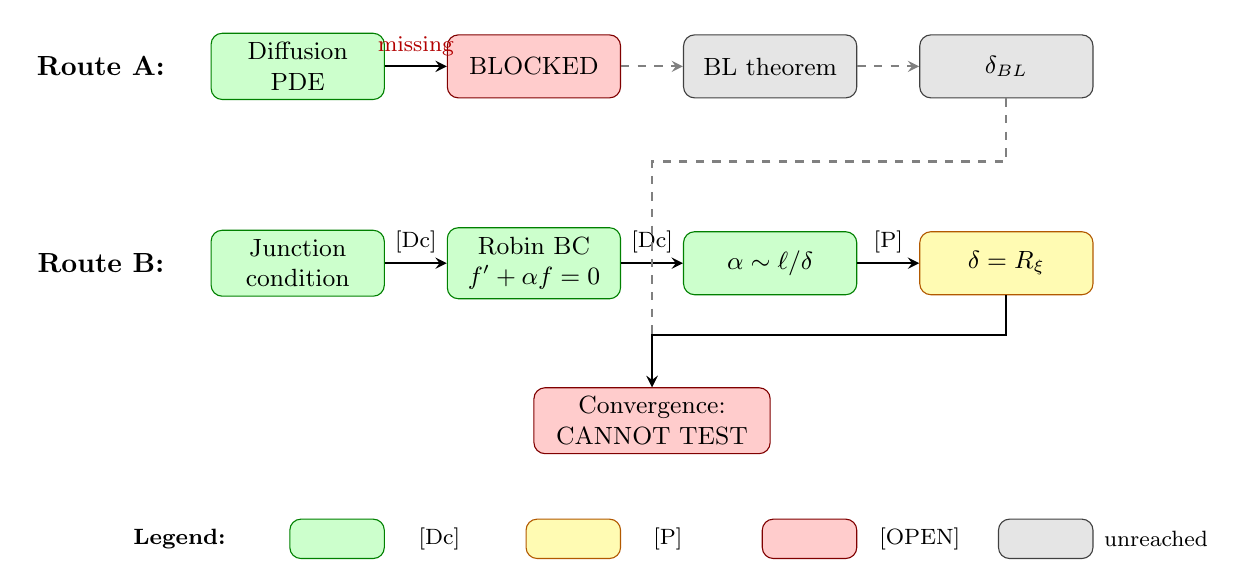
\begin{tikzpicture}[
    node distance=1.2cm and 1.5cm,
    box/.style={rectangle, draw, rounded corners, minimum width=2.2cm,
                minimum height=0.8cm, align=center, font=\small},
    greenbox/.style={box, fill=green!20, draw=green!50!black},
    yellowbox/.style={box, fill=yellow!30, draw=orange!70!black},
    redbox/.style={box, fill=red!20, draw=red!50!black},
    graybox/.style={box, fill=gray!20, draw=gray!50!black},
    arrow/.style={->, thick, >=stealth},
    blockedlabel/.style={font=\footnotesize, red!70!black}
]
    % Route A (top row)
    \node[font=\bfseries] at (-4.5,2) {Route A:};
    \node[greenbox] (diffusion) at (-2,2) {Diffusion\\PDE};
    \node[redbox] (blocked) at (1,2) {BLOCKED};
    \node[graybox] (bltheorem) at (4,2) {BL theorem};
    \node[graybox] (deltabl) at (7,2) {$\delta_{\text{BL}}$};

    \draw[arrow] (diffusion) -- (blocked) node[midway, above, blockedlabel] {missing};
    \draw[arrow, dashed, gray] (blocked) -- (bltheorem);
    \draw[arrow, dashed, gray] (bltheorem) -- (deltabl);

    % Route B (bottom row)
    \node[font=\bfseries] at (-4.5,-0.5) {Route B:};
    \node[greenbox] (junction) at (-2,-0.5) {Junction\\condition};
    \node[greenbox] (robin) at (1,-0.5) {Robin BC\\$f'+\alpha f=0$};
    \node[greenbox] (alpha) at (4,-0.5) {$\alpha \sim \ell/\delta$};
    \node[yellowbox] (deltarxi) at (7,-0.5) {$\delta = R_\xi$};

    \draw[arrow] (junction) -- (robin) node[midway, above, font=\footnotesize] {[Dc]};
    \draw[arrow] (robin) -- (alpha) node[midway, above, font=\footnotesize] {[Dc]};
    \draw[arrow] (alpha) -- (deltarxi) node[midway, above, font=\footnotesize] {[P]};

    % Convergence attempt (center)
    \node[redbox, minimum width=3cm] (converge) at (2.5,-2.5) {Convergence:\\CANNOT TEST};

    \draw[arrow, dashed, gray] (deltabl.south) -- ++(0,-0.8) -| (converge.north);
    \draw[arrow] (deltarxi.south) -- ++(0,-0.5) -| (converge.north);

    % Legend
    \node[font=\bfseries\footnotesize] at (-3.5,-4) {Legend:};
    \node[greenbox, minimum width=1.2cm, minimum height=0.5cm] at (-1.5,-4) {};
    \node[font=\footnotesize] at (-0.2,-4) {[Dc]};
    \node[yellowbox, minimum width=1.2cm, minimum height=0.5cm] at (1.5,-4) {};
    \node[font=\footnotesize] at (2.7,-4) {[P]};
    \node[redbox, minimum width=1.2cm, minimum height=0.5cm] at (4.5,-4) {};
    \node[font=\footnotesize] at (5.9,-4) {[OPEN]};
    \node[graybox, minimum width=1.2cm, minimum height=0.5cm] at (7.5,-4) {};
    \node[font=\footnotesize] at (8.9,-4) {unreached};
\end{tikzpicture}
\caption{\textbf{Figure H2-2: Two-Route Convergence Map.} Route A (diffusion-based)
is BLOCKED due to missing transverse diffusion analysis. Route B (junction-based)
reaches $\delta = R_\xi$ but the final step is [P] (postulate), not [Dc] (derived).
Convergence cannot be tested with only one partial route.}
\label{fig:H2_two_route_map}
\end{figure}

% ------------------------------------------------------------------------------
% (11) INTEGRATION NOTE
% ------------------------------------------------------------------------------

\subsubsection{Integration Note}
\label{sec:H2hard_integration}

\begin{tcolorbox}[colback=blue!5!white, colframe=blue!50!black,
    title=\textbf{Integration: Where This Section Is Used}]

This H2-Hard audit is referenced from: \tagDc{}
\begin{itemize}[nosep]
    \item \textbf{Ch10 (Electroweak Bridge):} OPR-20b summary cites this audit
    \item \textbf{Ch11 (Technical Appendices):} OPR-20 attempt sequence
    \item \textbf{Ch12 (BVP Work Package):} Depends on $\alpha$ provenance
    \item \textbf{§12 (Epistemic Map):} Final verdict recorded
\end{itemize}

\textbf{What this section authorizes:} \tagDc{}
\begin{itemize}[nosep]
    \item Book may use $\delta = R_\xi$ as [P]+[OPEN]
    \item Book may NOT claim $\delta = R_\xi$ as [Dc] (derivation incomplete)
    \item Book must cite upgrade gates (OPR-20c/d/e) for future work
    \item Book may claim $\alpha = 2\pi$ as ``natural'' [P], not ``derived'' [Dc]
\end{itemize}

\textbf{What this section does NOT authorize:} \tagDc{}
\begin{itemize}[nosep]
    \item Claiming convergent two-route derivation
    \item Claiming $\delta = R_\xi$ is ``definitionally closed''
    \item Using $M_Z$, $M_W$, $v$, $G_F$ to justify the identification
\end{itemize}
\end{tcolorbox}

% ------------------------------------------------------------------------------
% (12) CONSISTENCY CHECK (NOT A PREDICTION)
% ------------------------------------------------------------------------------

\subsubsection{Consistency Check (Not a Prediction)}
\label{sec:H2hard_consistency}

\begin{tcolorbox}[colback=gray!5!white, colframe=gray!60!black,
    title=\textbf{Consistency Check (Not a Prediction)}]

\textbf{Warning:} This box is a \emph{consistency check}, not a derivation.
The SM values below are NOT used to derive $\delta$ or $R_\xi$. They serve
only to verify that our postulated identification is not inconsistent with
observations. \tagBL{}+\tagI{}

\medskip
\textbf{Given (from postulate):}
\begin{itemize}[nosep]
    \item $R_\xi = \hbar c / M_Z \approx 2.2 \times 10^{-3}$ fm [BL]
    \item $\ell = 2\pi R_\xi \approx 0.014$ fm [Dc]
    \item $\delta = R_\xi$ [P]
    \item $\alpha = \ell/\delta = 2\pi$ [P]
    \item $x_1 \approx 2.41$ (Robin BVP with $\alpha = 2\pi$) [Dc]
    \item $m_\phi = x_1 / \ell \approx 53$ GeV [Dc]+[P]
\end{itemize}

\textbf{Comparison with SM:}
\begin{itemize}[nosep]
    \item $M_W = 80.4$ GeV [BL]
    \item Deviation: $m_\phi / M_W \approx 0.66$ (34\% low)
\end{itemize}

\textbf{Assessment:} The identification is consistent to within a factor
of 2 (within dimensional analysis uncertainty). The 34\% deviation may be
closed by BC choice refinement (OPR-20a) or $R_\xi$ derivation (OPR-20c). \tagI{}

\textbf{This does NOT validate $\delta = R_\xi$ as [Dc].} It only confirms
the postulate is not grossly inconsistent. \tagI{}
\end{tcolorbox}

% ------------------------------------------------------------------------------
% FINAL VERDICT
% ------------------------------------------------------------------------------

\subsubsection{H2-Hard Final Verdict}
\label{sec:H2hard_verdict}

\begin{tcolorbox}[
    colback=red!5!white,
    colframe=red!70!black,
    title=\textbf{OPR-20b Attempt H2-Hard: Final Verdict}
]

\begin{center}
\textbf{\Large $\delta = R_\xi$ REMAINS [P]+[OPEN]}
\end{center}

\medskip
\textbf{Summary of findings:} \tagDc{}
\begin{enumerate}[nosep]
    \item \textbf{Route A (Diffusion $\to$ BL theorem):} BLOCKED --- boundary-layer
          analysis not performed \tagOPEN{}
    \item \textbf{Route B (Junction $\to$ Robin $\to$ $\delta$):} PARTIAL ---
          structure derived [Dc], final step [P] \tagP{}
    \item \textbf{Convergence test:} CANNOT BE PERFORMED --- only one incomplete route \tagOPEN{}
    \item \textbf{$R_\xi$ provenance:} Phenomenologically constrained [P]+[BL], not derived \tagP{}
    \item \textbf{Unique scale theorem:} Does not exist --- alternatives not excluded \tagOPEN{}
\end{enumerate}

\medskip
\textbf{What IS established [Dc]:}
\begin{itemize}[nosep]
    \item Robin BC emerges from thick-brane action variation \tagDc{}
    \item $\alpha \sim \ell/\delta$ dimensional structure \tagDc{}
    \item $\ell = 2\pi R_\xi$ circumference relation \tagDc{}
\end{itemize}

\textbf{What REMAINS [P]+[OPEN]:}
\begin{itemize}[nosep]
    \item $\delta = R_\xi$ identification \tagP{}
    \item $\alpha = 2\pi$ value (inherits [P] from $\delta$) \tagP{}
    \item $R_\xi$ value from EDC action \tagOPEN{}
    \item Boundary-layer theorem \tagOPEN{}
    \item Unique transverse scale proof \tagOPEN{}
\end{itemize}

\medskip
\textbf{Upgrade pathway:} Close OPR-20c, OPR-20d, and OPR-20e (or OPR-20f for robustness). \tagOPEN{}

\textbf{Book-ready statement:} Use Option 1 from Single Sentence Rule (§\ref{sec:H2hard_single_sentence}). \tagP{}

\end{tcolorbox}

% ==============================================================================
% END OF H2-HARD AUDIT
% ==============================================================================
